% D.18 正方形 ABCD 边 4，E 为 BC 中点（CE=2，BE=2），F∈CD 且 CF=1
\documentclass[tikz,border=4pt]{standalone}
\usepackage{ctex}
\usepackage{amsmath}
\usetikzlibrary{calc}
\begin{document}
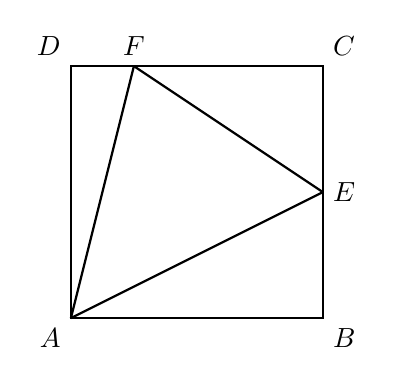
\begin{tikzpicture}[scale=0.8, thick]
  \coordinate (A) at (0, 0);
  \coordinate (B) at (4, 0);
  \coordinate (C) at (4, 4);
  \coordinate (D) at (0, 4);
  \coordinate (E) at (4, 2);
  \coordinate (F) at (1, 4);

  \draw (A) -- (B) -- (C) -- (D) -- cycle;
  \draw (A) -- (E);
  \draw (E) -- (F);
  \draw (A) -- (F);

  \node[below left]  at (A) {$A$};
  \node[below right] at (B) {$B$};
  \node[above right] at (C) {$C$};
  \node[above left]  at (D) {$D$};
  \node[right]       at (E) {$E$};
  \node[above]       at (F) {$F$};
\end{tikzpicture}
\end{document}
